\chapter{Proces konfiguracji modułów logiki programowalnej i systemu operacyjnego PetaLinux}
\label{cha:vivado-conf}



Użycie funkcjonalności opisywanych w niniejszej pracy wymaga przeprowadzenia konfiguracji wykorzystywanych modułów logicznych oraz systemu operacyjnego. 
W poniższych podrozdziałach zebrano informacje związane z poruszanymi zagadnieniami. 
Przedstawiono proces konfiguracji bazowego projektu Vivado i wykorzystania go na etapie budowy systemu PetaLinux, a także omówiono proces użycia modułów AXI i wybranych funkcjonalności systemu PetaLinux -- obliczeń równoległych, biblioteki OpenCV, mechanizmu przerwań systemowych.
Przedstawiono również proces konfiguracji modułu generacji tła zaproponowanego w rozdziale \ref{cha:project}.

Omawiane zagadnienia wymagają użycia oprogramowania Vivado \cite{vivado-home} i zintegrowanego z nim środowiska programistycznego Xilinx SDK \cite{xsdk-home}. Ponadto, konfiguracja systemu operacyjnego odbywa się przy użyciu narzędzi pakietu PetaLinux Tools \cite{petalinux-tools}.

\section{Podstawowa konfiguracja projektu}
\label{sec:basic-proj-config}
Wykorzystana w projekcie karta -- Digilent ZYBO -- nie jest bezpośrednio wspierana przez środowisko Vivado.
Wynika z tego konieczność sprecyzowania parametrów układu na etapie tworzenia projektu. 
W trakcie modyfikowania projektu, w przypadku dodania modułów wykorzystujących interfejs wejścia/wyjścia, konieczna jest również konfiguracja parametrów interfejsu. 
Aby uprościć proces projektowania, zalecane jest skonfigurowanie obsługi układu przed utworzeniem projektu. 
Proces ten opisano w dokumentacji producenta \cite{zybo-in-vivado}.

\subsection{Vivado}
\label{sec:vivado-conf}
Utworzyć należy projektu typu \emph{,,RTL Project''}, z odznaczoną opcją \emph{,,Do not specify sources at this time''}.
W kroku \emph{,,Add Constraints''} dodać należy plik konfiguracyjny dla wybranego układu. 
W przypadku ZYBO, plik ten jest dostępny na stronie producenta. 
W kolejnym kroku możliwe jest skonfigurowanie parametrów układu. 
Wykorzystać do tego należy zakładkę \emph{,,Boards''} i wybrać wykorzystywany model.

Po utworzeniu projektu, skonfigurować należy właściwą przestrzeń roboczą dla projektu, wykorzystując do tego opcję \emph{,,IP Integrator --> Create Block Design''}.
Do nowo utworzonej przestrzeni dodać należy moduł IP reprezentujący procesor ZYNQ -- \emph{,,ZYNQ7 Processing System''}.
W kolejnych krokach należy dokonać konfiguracji modułu procesora, klikając dwukrotnie na moduł.

\begin{itemize}
	\item Kanały interfejsu AXI mogą być konfigurowane przez zakładkę \emph{,,PS-PL Configuration''}. Możliwa jest aktywacja kanałów ogólnego przeznaczenia (\emph{GP}) oraz wysokiej wydajności (\emph{HP}).
	
	\item Interfejsy komunikacji konfigurowane mogą być z poziomu zakładki \emph{,,MIO Configuration''}. Zalecane jest aktywowanie interfejsów \emph{ENET 0}, \emph{SD 0} i \emph{UART 1} ze względu na ich wykorzystanie na dalszym etapie pracy.
	
	Przykład konfiguracji interfejsów wejścia/wyjścia przedstawiono na rysunku \ref{fig:vivado-mio-configuration}.
	\begin{figure}[ht]
		\centering
		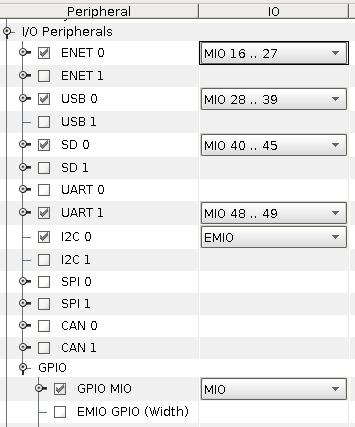
\includegraphics[height=8cm]{img/vivado/mio-configuration.png}
		\caption{Okno konfiguracji interfejsów wejścia i wyjścia.}
		\label{fig:vivado-mio-configuration}
	\end{figure}
	
	\item Parametry sygnałów zegarowych dostępnych z poziomu układów logiki reprogramowalnej modyfikować można w zakładce \emph{,,Clock Configuration/PL Fabric Clocks''}. W projekcie projekcie wymagającym obsługi AXI VDMA wykorzystano trzy sygnały zegarowe:
	\begin{itemize}[label=\textbullet]
		\item bazowy, o częstotliwości $100$MHz,
		\item wykorzystywany do komunikacji interfejsem AXI, o częstotliwości $140$MHz,
		\item zegar obsługi sekwencji wizyjnej, o częstotliwości $200$MHz, umożliwiający współpracę ze strumieniem wideo o częstotliwości $60$Hz i rozdzielczości co $1920 \times 1080$ pikseli.
	\end{itemize}
	
	\item Częstotliwość pracy procesora oraz pamięci zmienić można w zakładce \emph{,,Clock Configuration/Processor/Memory Clocks''}. Zdefiniować należy częstotliwość pracy CPU równą $650$MHz oraz DRR równą $525$MHz.
	
\end{itemize}

Po ukończeniu etapu konfiguracji procesora i powrocie do głównego okna programu, należy użyć opcji \emph{,,Run Block Automation''}. 
Utworzone zostaną połączenia interfejsów pamięci \texttt{DDR} oraz \texttt{FIXED\_IO}.
W przypadku zdefiniowania interfejsów AXI, połączyć należy właściwe sygnały zegarowe. 
Przykład wynikowej konfiguracji projektu przedstawiono na rysunku \ref{fig:vivado-config-result}.

	\begin{figure}[ht]
		\centering
		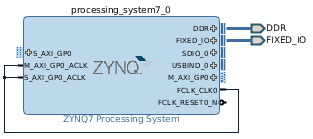
\includegraphics[]{img/vivado/vivado-config-result.png}
		\caption{Okno projektu.}
		\label{fig:vivado-config-result}
	\end{figure}
	
Przedstawiona konfiguracja stanowi podstawę każdego projektu wykorzystującego moduł procesora Zynq.
Po zakończeniu konfiguracji, wygenerować należy warstwę HDL, korzystając z opcji \emph{,,Create HDL Wrapper''} dostępnej po kliknięciu prawym przyciskiem myszy na utworzony wcześniej plik źródłowy.
Skonfigurowany w ten sposób projekt może być budowany i uruchamiany na platformie Zybo.

\subsection{SDK}

W celu utworzenia projektu aplikacji w SDK, konieczne jest wyeksportowanie plików opisujących projekt z poziomu Vivado, wykorzystując do tego opcję \emph{,,File/Export/Export Hardware''} z zaznaczoną opcją \emph{,,Include bitstream''}.
W efekcie, dostępny powinien być projekt \texttt{\textit{nazwa\_projektu}\_hw\_platform\_0}, zawierająca plik \texttt{nazwa\_projektu.hdf}, zawierający konfigurację sprzętową, stanowiący podstawę każdego budowanego programu \textit{bare-metal}. 

W przypadku budowania aplikacji na platformę PetaLinux, na etapie tworzenia projektu, zmodyfikować należy pole \emph{,,OS Platform''} na wartość \emph{,,linux''}, \emph{,,Processor Type''} na \emph{,,ps7\_cortexa9''} oraz wybrać właściwy język programowania.
Tak zdefiniowana aplikacja nie może korzystać z bibliotek udostępnianych przez firmę \emph{Xilinx} )(na przykład zawierających procedury obsługi modułów VDMA czy kontrolera przerwań), ale mogą korzystać z pełnej biblioteki standardowej jeżyka \emph{C} oraz rozszerzeń \emph{POSIX}, w tym operacji wejścia/wyjścia, komunikacji sieciowej czy bibliotek matematycznych.


W celu uruchomienia aplikacji systemowej na platformie ZYBO, przeprowadzić należy proces budowania i skopiować wynikowy plik z katalogu \texttt{Debug} lub \texttt{Release} do systemu plików systemu PetaLinux. 
Wykorzystać można do tego narzędzie SSH:

\begin{lstlisting}[breaklines=true]
scp Debug/hello-world.elf root@adres-ip:~/
\end{lstlisting}

Aplikację uruchomić można przy użyciu konsoli użytkownika, również stosując narzędzie SSH.

\subsection{PetaLinux}
\label{sec:petalinux-config}

%TODO - a tu nie trzeba zrobić czegoś wcześniej ? Pobrać zainstalowć itp ?
% nie opisywałem procesu instalacji Vivado, uznałem więc, że nie ma też powodu by opisywać instalację petalinux. Dodam na początku rozdziału informację o wykorzystywanych narzędziach
%TODO Vivado to proste, ale o tym PetaLinux to bym coś napisał....

Utworzenie struktury katalogów projektu wykonywane jest przy użyciu poniższego polecenia.

\begin{lstlisting}[breaklines=true]
petalinux-create -t project --template zynq --name (*@\textit{nazwa-projektu}@*)
cd (*@\textit{nazwa-projektu}@*)
\end{lstlisting}

Powstała struktura zintegrowana jest z systemem kontroli wersji \emph{git}, co pozwala zachować uporządkowanie danych wewnątrz projektu oraz wersjonowanie. 
Kolejnym krokiem jest zaimportowanie projektu \emph{Vivado}.

\begin{lstlisting}[breaklines=true]
petalinux-config --get-hw-description=(*@\textit{/sciezka/do/projektu/projekt.sdk/}@*)
\end{lstlisting}

Jeśli polecenie wywołane zostało po raz pierwszy dla danego projektu, uruchomione zostanie narzędzie konfiguracyjne, domyślne ustawienia są jednak poprawne.
Konfiguracja projektu odbywa się przy użyciu polecenia \texttt{petalinux-config}.
Skonfigurować należy metodę uruchamiania systemu -- w omawianym przypadku, uruchomienie następuje na bazie plików znajdujących się na karcie SD.
\begin{lstlisting}[breaklines=true]
petalinux-config
Image Packaging Configuration -> Root filesystem type -> SD card
\end{lstlisting}

Należy również zmodyfikować argumenty przekazywane systemowi na etapie uruchamiania, umożliwiając wykorzystanie sterowników do modułów logiki reprogramowalnej.

\begin{lstlisting}[breaklines=true]
petalinux-config
Kernel Bootargs -> dezaktywować opcję Generate boot args automatically i zdefiniować własną wartość
console=ttyPS0,115200 earlyprintk uio_pdrv_genirq.of_id=generic-uio root=/dev/mmcblk0p2 rw rootwait 
\end{lstlisting}
Następnie, przeprowadzić należy proces budowania systemu oraz wygenerować pliki wynikowe.

\begin{lstlisting}[breaklines=true]
petalinux-build
petalinux-package --boot --fsbl images/linux/zynq_fsbl.elf --fpga images/linux/system_wrapper.bit --u-boot --force
petalinux-package --image -c rootfs --format initramfs
\end{lstlisting}

Uruchomienie systemu wymaga przygotowania karty SD -- musi ona posiadać dwie partycje, pierwszą, z etykietą \emph{boot} i systemem plików \emph{fat32}, drugą -- odpowiednio \emph{sys} i \emph{ext4}. 
Pierwsza z nich, zawierająca pliki wymagane na etapie inicjalizacji systemu, musi być poprzedzona 4 MB niezaalokowanej przestrzeni i mieć rozmiar co najmniej 40 MB. 
Druga partycja zawiera pliki systemowe, jej rozmiar powinien wynosić co najmniej kilkaset megabajtów. 
Proces formatowania przeprowadzić można przy użyciu narzędzia \emph{gparted}. Na rysunku \ref{fig:gparted-screen} przedstawiono efekt konfiguracji karty SD.

\begin{figure}[H]
	\centering
	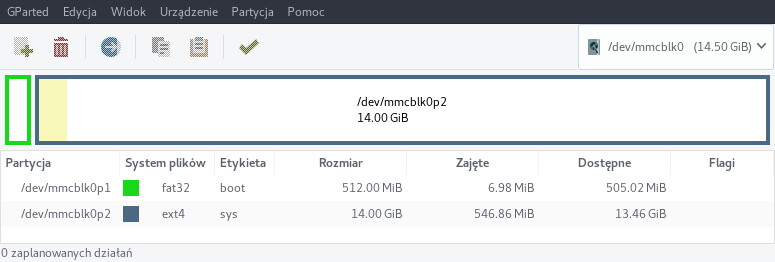
\includegraphics[width=12cm]{img/gparted-screen.png}
	\caption{Partycjonowane karty SD przy użyciu programu gparted.}
	\label{fig:gparted-screen}
\end{figure}

Pliki wynikowe należy przenieść na kartę SD, korzystając z poniższych poleceń.

\begin{lstlisting}[breaklines=true]
rm -rf /(*@\textit{punkt-montowania}@*)/sys/*
cp images/linux/BOOT.BIN /(*@\textit{punkt-montowania}@*)/boot/
cp images/linux/image.ub /(*@\textit{punkt-montowania}@*)/boot/
cp images/linux/rootfs.cpio /(*@\textit{punkt-montowania}@*)/sys/
cd /(*@\textit{punkt-montowania}@*)/
pax -rvf rootfs.cpio
sync
cd -
\end{lstlisting}

Ze względu na mechanizm buforowania przez kontroler operacji zapisu danych, pamiętać należy o wywołaniu polecenia \texttt{sync}, zapewniającego zachowanie integralności danych.
Karta SD pozwala na uruchomienie systemu operacyjnego na układzie i przechowywanie danych użytkownika pomiędzy startami układu. 
Dalsza praca z systemem odbywać się może przez protokoły komunikacji \emph{SSH} lub \emph{UART}.

\section{Konfiguracja modułu wykorzystującego interfejs AXI}
\label{sec:vivado-axi-dma}

Interfejs AXI stanowi podstawową metodę komunikacji pomiędzy modułami logiki programowalnej oraz elementami FPGA i CPU. 
Dzięki wykorzystaniu tego protokołu do obsługi projektowanych narzędzi, możliwe jest użycie zbioru elementów dostępnych w bibliotece Vivado i uproszczenie procesu projektowania procedur komunikacyjnych. 
Poniżej przedstawiono kroki konfiguracyjne wewnątrz narzędzi Vivado i PetaLinux.

\subsection{Vivado}
Oprogramowanie Vivado umożliwia zbudowanie modułu wykorzystującego protokół AXI przez użycie opcji \emph{,,Create and package new IP...''}, zawartej w menu \emph{Tools}.
Na ekranie wyboru zadania wybrać należy opcję \emph{,,Create a new AXI4 peripheral''}.
Po zdefiniowaniu podstawowych danych związanych z modułem, takich jak jego nazwa i nazwisko autora, w kolejnym kroku możliwe będzie zdefiniowanie interfejsu modułu. 
Na tym etapie konfiguracji dodać należy wszystkie połączenia wykorzystujące interfejs AXI. 
W przypadku modułu konfiguracyjnego o podstawowej strukturze, interfejs zawierać powinien jedno połączenie wykorzystujące protokół AXI w wersji \emph{Lite}, działający w trybie \emph{slave}, z oczekiwaną liczbą rejestrów. 
Każdy rejestr powinien być związany z jedną wartością, której konfiguracja ma być możliwa. 
Przykład konfiguracji przedstawiono na rysunku \ref{fig:axi-dma-interfaces-conf}.


\begin{figure}[H]
	\centering
	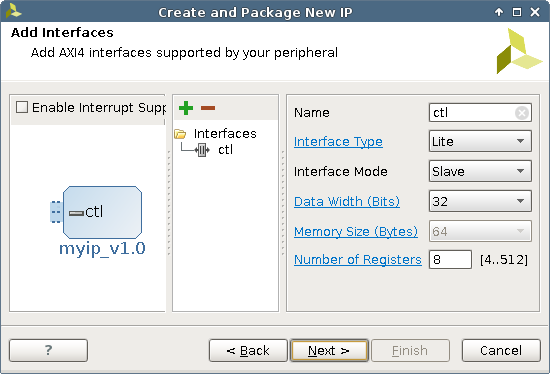
\includegraphics[width=8cm]{img/vivado/axi-dma-interfaces-conf.png}
	\caption{Konfiguracja interfejsów modułu AXI DMA.}
	\label{fig:axi-dma-interfaces-conf}
\end{figure}

W omawianym przykładzie zdefiniowano interfejs AXI o nazwie \emph{ctl}, związany z ośmioma rejestrami o długości trzydziestu dwóch bitów w pamięci.
Zdefiniowanie interfejsów kończy proces podstawowej konfiguracji modułu. W kolejnym kroku należy wybrać opcję \emph{,,Edit IP''} w celu dostosowania kodu źródłowego modułu.

Po wygenerowaniu, z modułem powinien być związany jeden plik źródłowy, zwierający instrukcje odpowiadające za obsługę komunikacji przy użyciu interfejsu AXI.
Do pliku dodać należy elementy odpowiedzialne za zdefiniowanie wyjść modułu oraz przypisanie im właściwych wartości.
W celu zadeklarowania wyjść modułu, odpowiadające im wpisy należy umieścić po komentarzu \emph{,,// Users to add ports here''}. Przykład przedstawiono na listingu \ref{listing:axi-dma-outputs}.

\begin{lstlisting}[breaklines, label=listing:axi-dma-outputs, caption=Definicja interfejsów wyjściowych modułu.]
// Users to add ports here
output wire parameter_a,
output wire [7:0] parameter_b,
output wire [15:0] parameter_c,
output wire [31:0] parameter_d,
// User ports ends
\end{lstlisting}

Zdefiniowano cztery sygnały wyjściowe, o różnej liczbie bitów.
Następnie, należy dokonać modyfikacji kodu odpowiedzialnego za powiązanie wartości parametrów z rejestrami modułu. 
Rejestry AXI zdefiniowane są poniżej linii \emph{,,//-- Number of Slave Registers N''}, gdzie \emph{N} to liczba dostępnych rejestrów. Rejestry te mają nazwy \texttt{slv\_reg\emph{n}}, gdzie \emph{n} to indeks rejestru -- nie jest zalecana modyfikacja tych nazw.
Modyfikacji kodu należy dokonać poniżej linii \emph{,,// Add user logic here''}. 
Przykład przedstawiono na listingu \ref{listing:axi-dma-associate}.

\begin{lstlisting}[breaklines, label=listing:axi-dma-associate, caption=Powiązanie wyjść z rejestrami modułu.]
// Add user logic here
assign parameter_a = slv_reg0[0];
assign parameter_b = slv_reg1[7:0];
assign parameter_c = slv_reg2[15:0];
assign parameter_d = slv_reg3[31:0];
// User logic ends
\end{lstlisting}

Wartości parametrów powiązano bezpośrednio z danymi znajdującymi się w rejestrach. 
W rozbudowanych aplikacjach może być konieczne dodanie instrukcji modyfikujących wartości rejestrów przed przesłaniem ich na wyjście modułu.
Po ukończeniu modyfikacji modułu, konieczne jest zapisanie zmian i wygenerowanie plików wynikowych. 
W tym celu należy wykorzystać okno \emph{,,Package IP''}, sekcję \emph{,,Review and Package''}. 
Widok narzędzia przedstawiono na rysunku \ref{fig:axi-dma-review-package}.

\begin{figure}[ht]
	\centering
	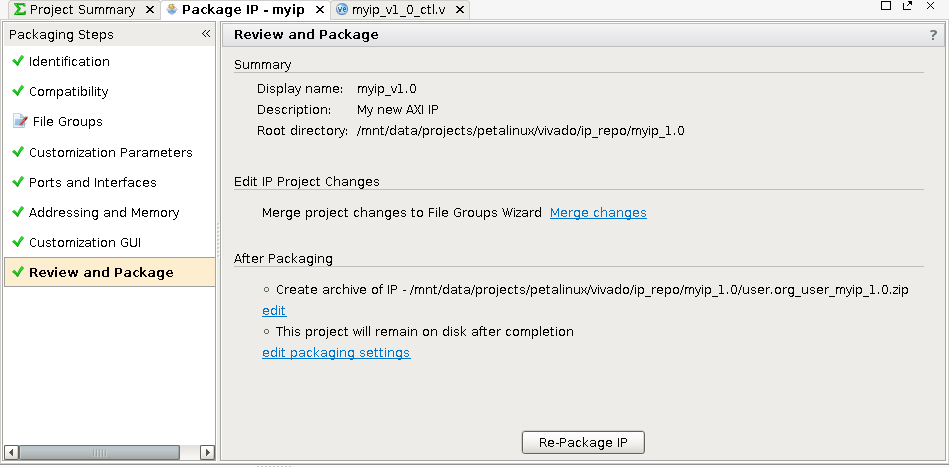
\includegraphics[width=12cm]{img/vivado/axi-dma-review-package.png}
	\caption{Okno finalizacji modyfikacji modułu.}
	\label{fig:axi-dma-review-package}
\end{figure}

Należy wybrać opcję \emph{,,Merge changes''}, umożliwiającą zintegrowanie wprowadzonych zmian z projektem bazowym. 
Następnie, można zakończyć edycję projektu przez wybór opcji \emph{,,Re-Package IP''}. 
Moduł będzie dostępny z poziomu interfejsu wyszukiwania modułów IP.
Dodanie modułu do projektu wymaga zdefiniowania adresu pamięci z nim związanego. Wykorzystać do tego należy okno \emph{,,Address Editor''}, dostępną w z poziomu głównego okna projektu. W omawianym przykładzie, z modułem powiązano przestrzeń rozpoczynającą się od adresu \texttt{0x43000000} i długości \texttt{64K}.
\subsection{SDK}
\label{sec:vivado-axi-dma-sdk}

Konfiguracja wartości parametrów modułu opiera się na zapisie pod właściwe adresy pamięci. 
W przypadku pracy w trybie \textit{bare-metal}, wykorzystać można instrukcję \emph{Xil\_Out32} z biblioteki \emph{xil\_io.h}. 
W przypadku pracy z systemem PetaLinux, wykorzystać należy biblioteki systemowe. 
Implementację \textit{bare-metal} przedstawiono na listingu \ref{lis:axi-dma-bare-metal}, natomiast systemową na listingach \ref{lis:axi-dma-petalinux-main}, \ref{lis:axi-dma-petalinux-axi-h} i \ref{lis:axi-dma-petalinux-axi-c}.

\begin{lstlisting}[breaklines, language=C, label=lis:axi-dma-bare-metal, caption=Obsługa modułu w trybie bare-metal.]
#include "xparameters.h"
#include "platform.h"
#include "xil_io.h"

#define PARAMETER_A_REGISTER 0
#define PARAMETER_B_REGISTER 4
#define PARAMETER_C_REGISTER 8
#define PARAMETER_D_REGISTER 12

#define BASEADDR XPAR_ALGORITHM_PARAMETERS_0_CTL_BASEADDR

int main()
{
	init_platform();
	
	Xil_Out32(BASEADDR + PARAMETER_A_REGISTER, 1);
	Xil_Out32(BASEADDR + PARAMETER_B_REGISTER, 25);
	Xil_Out32(BASEADDR + PARAMETER_C_REGISTER, 1 << 10);
	Xil_Out32(BASEADDR + PARAMETER_D_REGISTER, 1 << 30);
	
	while(1);
}
\end{lstlisting}


\begin{lstlisting}[breaklines, language=C, label=lis:axi-dma-petalinux-main, caption=Obsługa modułu w trybie systemowym - \texttt{main.c}.]
#include <fcntl.h>
#include <stdio.h>
#include <stdlib.h>
#include <sys/mman.h>

#include "axi.h"

#define PARAMETER_A_REGISTER 0
#define PARAMETER_B_REGISTER 4
#define PARAMETER_C_REGISTER 8
#define PARAMETER_D_REGISTER 12

#define BASEADDR 0x43000000

typedef int memory_handle_t;

void setup_virtual_memory(struct axi_interface *interface, size_t length, memory_handle_t memory_handle, off_t base_addr) {
	interface->base_addr = base_addr;
	interface->virt_addr = (virt_address) mmap(NULL, length, PROT_READ | PROT_WRITE, MAP_SHARED, memory_handle, base_addr);
	if (interface->virt_addr == MAP_FAILED) {
		perror("Failed to map virtual memory.");
		exit(1);
	}
}

int main() {
	memory_handle_t memory_handle = open("/dev/mem", O_RDWR | O_SYNC);
	
	struct axi_interface* parameters = (struct axi_interface*) malloc(sizeof(struct axi_interface));
	if (parameters == NULL) {
		perror("Memory allocation failed.");
		exit(1);
	}
	setup_virtual_memory(parameters, 65535, memory_handle, BASEADDR);
	
	axi_write(parameters->virt_addr, PARAMETER_A_REGISTER, 1);
	axi_write(parameters->virt_addr, PARAMETER_B_REGISTER, 25);
	axi_write(parameters->virt_addr, PARAMETER_C_REGISTER, 1 << 10);
	axi_write(parameters->virt_addr, PARAMETER_D_REGISTER, 1 << 30);
	
	unsigned int parameter_a = axi_read(parameters->virt_addr, PARAMETER_A_REGISTER);
	
	while(1);
}
\end{lstlisting}

\begin{lstlisting}[breaklines, language=C, label=lis:axi-dma-petalinux-axi-h, caption=Obsługa modułu w trybie systemowym - \texttt{axi.h}.]
typedef unsigned int* virt_address;

struct axi_interface {
	unsigned int base_addr;
	virt_address virt_addr;
};

void axi_write(virt_address virt_addr, int location, unsigned int value);
unsigned int axi_read(virt_address virt_addr, int location);
\end{lstlisting}

\begin{lstlisting}[breaklines, language=C, label=lis:axi-dma-petalinux-axi-c, caption=Obsługa modułu w trybie systemowym - \texttt{axi.c}.]
#include "axi.h"

void axi_write(virt_address virt_addr, int location, unsigned int value) {
	virt_addr[location >> 2] = value;
}

unsigned int axi_read(virt_address virt_addr, int location) {
	return virt_addr[location >> 2];
}
\end{lstlisting}


System Linux udostępnia zbiór procedur związanych z obsługą pamięci operacyjnej, w tym pozwalające na wirtualizację fizycznych adresów, co jest konieczne do obsługi urządzeń peryferyjnych z poziomu systemu operacyjnego.
Adres fizyczny urządzenia zdefiniowano przez nazwę \texttt{BASEADDR}. Określono również przesunięcia adresów kolejnych rejestrów modułu, na przykład \texttt{PARAMETER\_A\_REGISTER}.

Procedura \texttt{setup\_virtual\_memory} przyjmuje jako argumenty wskaźnik do struktury interfejsu AXI, zawierającej informacje o adresach fizycznym i wirtualnym pamięci, rozmiarze przestrzeni adresowej w bajtach, a także uchwyt do kontrolera pamięci systemowej oraz adres fizyczny modułu.
W wyniku konfiguracji obszar pamięci fizycznej mapowany jest w przestrzeni adresowej systemu, co pozwala na odczyt i zapis wartości.
Aby uprościć mechanizm odczytu i zapisu do pamięci, udostępniono procedury \texttt{axi\_write} i \texttt{axi\_read}, których argumentami wywołań jest bazowy adres wirtualny modułu oraz przesunięcie wybranego rejestru.

Poprawność działania komunikacji przetestowano na przykładzie modułu liczącego, kontrolowanego z poziomu systemu operacyjnego. 
Moduł udostępniał rejestr kontrolny, którego najmłodszy bit odpowiadał za aktywację pracy licznika, oraz rejestr przechowujący zliczaną wartość. Zapisując i odczytując wartości rejestrów zweryfikowano, że komunikacja z modułem ma prawidłowy przebieg.

\subsection{PetaLinux}
\label{sec:vivado-axi-dma-petalinux}

W celu wykorzystania techniki DMA w aplikacji działającej w systemie PetaLinux, konieczna jest aktywacja właściwych parametrów konfiguracji na etapie budowania systemu. 
W tym celu wykonać należy polecenie:

\begin{lstlisting}[breaklines]
petalinux-config -c kernel
\end{lstlisting}

i aktywować funkcjonalność DMA:

\begin{lstlisting}[breaklines]
Device Drivers -> DMA Engine Support
Device Drivers -> DMA Engine Support -> Xilinx AXI DMAS Engine
\end{lstlisting}

Włączenie sterowników DMA oraz zmodyfikowanie argumentów uruchomienia systemu operacyjnego, opisane w rozdziale \ref{sec:petalinux-config}, pozwala na wykorzystanie interfejsu AXI i techniki DMA do komunikacji z modułami logiki programowalnej.



\section{Konfiguracja modułu AXI VDMA}
\label{sec:vivado-axi-vdma}

Proces konfiguracji modułu VDMA składa się z kroków podobnych do opisanych w rozdziale \ref{sec:vivado-axi-dma}, poświęconej modułom AXI DMA. Poniżej przedstawiono dodatkowe kroki, związane bezpośrednio z konfiguracją modułu VDMA.

\subsection{Vivado}
Do projektu dołączyć należy moduł \textit{AXI Video Direct Memory Access}. 
Okno konfiguracji związane z nim pozwala na wybór obsługiwanych kanałów:
\begin{itemize}
	\item write (\emph{S2MM}) -- kanał zapisu, pozwalający na transmisję danych z formatu strumieniowego do pamięci operacyjnej,
	\item read (\emph{MM2S}) -- kanał odczytu, umożliwiający konwersję danych przechowywanych w pamięci do strumienia.
\end{itemize}

Ustawienia pozwalają na wybór szerokości strumienia informacji dla jednego piksela, maksymalną liczbę buforów w pamięci oraz długość linii buforujących, związanych z oboma kanałami.
Wartości wielkości strumienia danych oraz liczby buforów związane są ściśle z projektowanym algorytmem, natomiast długość linii buforujących może wpłynąć na stabilność działania systemu. 
Zwiększenie tej wartości może poprawić działanie algorytmu w przypadku, gdy operacje związane z pamięcią operacyjną wykonywane są z opóźnieniem.

Zakładka ustawień zaawansowanych pozwala na zdefiniowanie parametrów związanych ze sterowaniem kanałami transmisji.
Wartość parametru \textit{,,Fsync Options''} w aplikacjach nie wymagających zewnętrznej synchronizacji powinna być zdefiniowana jako \texttt{tuser} dla kanału zapisu oraz \texttt{none} dla kanału odczytu, dzięki czemu sygnał synchronizacji modułu będzie związany z wejściowym strumieniem AXI. 
Część aplikacji może wymagać synchronizacji strumienia odczytu z drugim strumieniem danych, na przykład z inną ramką sygnału wizyjnego. 
W takiej sytuacji wykorzystać należy opcję synchronizacji \texttt{fsync}, a wejście układu \texttt{mm2s\_fsync} połączyć z właściwym sygnałem synchronizacji.

W ramach pracy wykorzystywano również synchronizację pomiędzy kanałami przy użyciu parametru \texttt{GenLock}, o wartości \texttt{master} dla kanału zapisu i \texttt{slave} dla odczytu. 
Pozwalało to zachować przesunięcie o stałej, definiowanej z poziomu aplikacji, wartości pomiędzy buforami wykorzystywanymi przez oba kanały.

Ze względu na dużą wartość przepływu danych przez oba kanały, do komunikacji z procesorem wykorzystać należy połączenia o wysokiej wydajności. Kanały te można aktywować korzystając z opcji konfiguracyjnych modułu \emph{ZYNQ7 Processing System}: \emph{,,PL-PS Configuration/HP Slave AXI Interface''}, i aktywując jeden lub wiele kanałów.
Z modułem AXI VDMA powiązać należy sygnał zegarowy o częstotliwości nie mniejszej od wartości tak zwanego zegara piksela, związanego ze strumieniem wizyjnym na wejściu. 
Sygnał ten powinien być generowany przez układ ZYNQ, a nie powiązany bezpośrednio z zegarem strumienia obrazu.

\subsection{SDK}
Konfiguracja modułu VDMA wymaga zastosowania technik opisanych w rozdziale \ref{sec:vivado-axi-dma-sdk}.

Proces uruchamiania transmisji dla modułu wymaga wykonania kroków zdefiniowanych przez producenta i opisanych w rozdziale \textit{,,Programming Sequence''} dokumentacji \cite{axi-vdma-guide}. Kod programu odpowiedzialnego za konfigurację modułu AXI VDMA przedstawiono na listingu \ref{lis:axi-vdma-sdk}.
\begin{lstlisting}[breaklines,language=C, label=lis:axi-vdma-sdk, caption=Obsługa modułu AXI VDMA w aplikacji \textit{bare-metal}.]
#include "xparameters.h"
#include "platform.h"
#include "xil_printf.h"
#include "xil_io.h"
#include "sleep.h"
#include "xaxivdma.h"

#define S2MM_VDMACR 0x30
#define S2MM_VDMASR 0x34
#define S2MM_VSIZE 0xA0
#define S2MM_HSIZE 0xA4
#define S2MM_FRMDLY_STRIDE 0xA8
#define S2MM_START_ADDRESS 0xAC
#define PART_PTR_REG 0x28
#define MM2S_VDMACR 0x00
#define MM2S_VDMASR 0x04
#define MM2S_VSIZE 0x50
#define MM2S_HSIZE 0x54
#define MM2S_FRMDLY_STRIDE 0x58
#define MM2S_START_ADDRESS 0x5C
#define HSIZE_FULL 1980
#define VSIZE_FULL 750

#define HSIZE_ACTIVE 1280
#define VSIZE_ACTIVE 720

#define PIXEL_SIZE 3
static volatile u8 framebuffer1[VSIZE_ACTIVE*HSIZE_ACTIVE*PIXEL_SIZE] = {0};
static volatile u8 framebuffer2[VSIZE_ACTIVE*HSIZE_ACTIVE*PIXEL_SIZE] = {0};
static volatile u8 framebuffer3[VSIZE_ACTIVE*HSIZE_ACTIVE*PIXEL_SIZE] = {0};

XAxiVdma AxiVdmaFrameBuffering;

void debug_vdma(UINTPTR addr);

void init_vdma_buffer(UINTPTR addr, u32 fb1, u32 fb2, u32 fb3)
{
	// 1
	Xil_Out32(addr + MM2S_VDMACR,
	(255 << 16) | 0x8 | 0x80 | 0x2 | 0x1);
	Xil_Out32(addr + S2MM_VDMACR,
	(255 << 16) | 0x8 | 0x80 | 0x2 | 0x1);
	
	// 2
	Xil_Out32(addr + MM2S_START_ADDRESS, fb1);
	Xil_Out32(addr + MM2S_START_ADDRESS + 4, fb2);
	Xil_Out32(addr + MM2S_START_ADDRESS + 8, fb3);
	
	Xil_Out32(addr + S2MM_START_ADDRESS, fb1);
	Xil_Out32(addr + S2MM_START_ADDRESS + 4, fb2);
	Xil_Out32(addr + S2MM_START_ADDRESS + 8, fb3);
	
	// 3
	Xil_Out32(addr + MM2S_FRMDLY_STRIDE,HSIZE_ACTIVE*PIXEL_SIZE);
	Xil_Out32(addr + S2MM_FRMDLY_STRIDE,HSIZE_ACTIVE*PIXEL_SIZE | (2 << 24));
	
	// 4
	Xil_Out32(addr + MM2S_HSIZE,HSIZE_ACTIVE*PIXEL_SIZE);
	Xil_Out32(addr + S2MM_HSIZE,HSIZE_ACTIVE*PIXEL_SIZE);
	
	// 5
	Xil_Out32(addr + S2MM_VSIZE,VSIZE_ACTIVE);
	Xil_Out32(addr + MM2S_VSIZE,VSIZE_ACTIVE);
}

int main()
{
	init_platform();
		
	xil_printf("Config - vdma\r\n");
	// vdma frame buffering
	init_vdma_buffer(XPAR_FRAME_BUFFER_VDMA_PREVIOUS_FRAME_BASEADDR,
	(u32)&framebuffer1, (u32)&framebuffer2, (u32)&framebuffer3);

	xil_printf("Config - done\r\n");
	while(1) {
		xil_printf("XPAR_FRAME_BUFFER_VDMA_PREVIOUS_FRAME\r\n");
		debug_vdma(XPAR_FRAME_BUFFER_VDMA_PREVIOUS_FRAME_BASEADDR);
		sleep(1);
	}
	cleanup_platform();
	return 0;
}
\end{lstlisting}



Funkcja \texttt{init\_vdma\_buffer} jest odpowiedzialna za przeprowadzenie konfiguracji modułu VDMA. 
Jej argumenty stanowią adres elementu VDMA oraz adresy trzech buforów obrazu. 
Zagwarantować należy, by przestrzeń zarezerwowana na każdy bufor była wystarczająca do przechowania pełnej ramki obrazu. 
W przypadku wykorzystania modułu VDMA do transmisji kontekstu związanego z każdym pikselem, zmodyfikować należy wartość \texttt{PIXEL\_SIZE} do liczby bajtów zajmowanej przez jeden piksel.

Procedura \texttt{init\_vdma\_buffer} wykonuje szereg operacji związanych z uruchomieniem transmisji sygnału dla obu kanałów niezależnie.
Przedstawione poniżej działania związane są z indeksami znajdującymi się wewnątrz komentarzy w listingu.
\begin{enumerate}
	\item Konfiguracja przerwań i uruchomienie kanału VDMA.
	W prezentowanym przykładzie, oba kanały skonfigurowano do działania w trybie cyklicznym, korzystającym naprzemiennie ze wszystkich buforów obrazu, z aktywowanym trybem synchronizacji \emph{Genlock} o wewnętrznym źródle sygnału.
	
	\item Przypisanie adresów buforów obrazu. Mogą być one wspólne lub unikalne dla każdego kanału.
	
	\item Zdefiniowanie parametrów obrazu wejściowego z sygnałami wygaszania i wzajemnego opóźnienia kanałów.
	W omawianym przykładzie, kanał odczytu zachowuje opóźnienie dwóch klatek obrazu względem kanału zapisu.
	
	\item Przypisanie rozmiaru jednej linii obrazu, z uwzględnieniem wielkości piksela w bajtach, nie uwzględniając cykli wygaszania.
	
	\item Zdefiniowanie liczby linii obrazu, nie uwzględniając cykli wygaszania.
\end{enumerate}

Wpisanie wartości do rejestrów \texttt{S2MM\_VSIZE} i \texttt{MM2S\_VSIZE} powoduje rozpoczęcie transmisji sygnału.

\subsection{Petalinux}
Konfiguracja projektu zgodna jest z opisem dla modułów DMA, przedstawionym w rozdziale \ref{sec:vivado-axi-dma-petalinux}. 
W przypadku projektu aplikacji działającej pod kontrolą systemu operacyjnego, pamiętać należy, że konfiguracja buforów obrazu wymaga użycia adresów fizycznych, które mogą różnić się od adresów wirtualnych komórek pamięci.

Zdefiniować należy adresy buforów, odległe od siebie co najmniej o rozmiar jednej ramki sygnału wizyjnego. 
Zagwarantować należy nienaruszalność pamięci z perspektywy systemu operacyjnego. 
Efekt ten najprościej jest osiągnąć przez ograniczenie rozmiaru pamięci dostępnej dla systemu operacyjnego i zdefiniowanie adresów buforów poza tym zakresem. 
Wykorzystać do tego można argument \textit{mem} przekazywany na etapie uruchamiania systemu, na przykład \texttt{mem=224M}. 
Proces dodawania argumentów uruchamiania systemu opisano w rozdziale \ref{sec:petalinux-config}. 

Adres fizyczny pamięci nie może być odczytany bezpośrednio, w tym celu musi zostać powiązany z adresem wirtualnym. 
Odpowiedzialną za to procedurę \texttt{setup\_virtual\_memory} przestawiono na listingu \ref{lis:axi-dma-petalinux-main}, przy czym parametr \texttt{base\_addr} to adres fizyczny pierwszej komórki bufora. 

\section{Obliczenia równoległe}
\label{sec:multithreading-config}
Użycie rozwiązań omawianych w rozdziale \ref{sec:openmp} wymaga aktywacji właściwych funkcji kompilacji.
W przypadku zastosowania wątków natywnych lub biblioteki dostępnej w standardzie C++ wymagane jest aktywowanie przełączników: 

\begin{lstlisting}[language=bash]
gcc main.c -o main.out (*@\textbf{-pthread}@*)
g++ main.cpp -o main.out (*@\textbf{-std=c++11}@*) (*@\textbf{-pthread}@*)
\end{lstlisting}

Dla biblioteki TBB wymagane jest przeprowadzenie linkowania względem jej kodu źródłowego:

\begin{lstlisting}[language=bash]
g++ main.cpp -o main.out (*@\textbf{-ltbb}@*)
\end{lstlisting}

Natomiast dla interfejsu OpenMP, konieczne jest użycie przełącznika:

\begin{lstlisting}[language=bash]
g++ main.cpp -o main.out (*@\textbf{-fopenmp}@*)
\end{lstlisting}

Wykorzystanie omawianych rozwiązań wiąże się z użyciem dedykowanych procedur lub dyrektyw kompilatora. 
Etap projektowania aplikacji działającej pod kontrolą systemu operacyjnego PetaLinux nie różni się od budowania oprogramowania na inne platformy. Należy jednak pamiętać, że układ Zynq wyposażony jest w procesor ARM o dwóch rdzeniach, więc potencjalne korzyści zastosowania aplikacji wielowątkowej nie przekraczają dwukrotnego zwiększenia szybkości działania aplikacji.
Sposób zastosowania bibliotek znaleźć można w dokumentacji każdego z narzędzi i literaturze cytowanej w związanym z tym zagadnieniem rozdziale.


\section{Biblioteka OpenCV}
\label{sec:opencv-config}
\subsection{OpenCV 2}
Biblioteka OpenCV w wersji 2.4 nie jest oficjalnie dostępna w pakiecie PetaLinux, może jednak zostać dołączona do systemu operacyjnego dzięki mechanizmowi aplikacji użytkownika.
Należy zatem przeprowadzić proces kompilacji kodu źródłowego biblioteki wraz z zależnościami, ponieważ prekompilowane pliki na platrofmę ARM nie są publicznie dostępne. Poniżej przedstawiono proces instalacji zależności.%

\begin{lstlisting}[breaklines=true, language=Bash, caption=Definicja zmiennych środowiskowych.]
export ARMPREFIX=(*@\textit{ścieżka/instalacji}@*)
export CCPREFIX=arm-linux-gnueabihf-
\end{lstlisting}

Zmienna \texttt{CCPREFIX} wskazuje na prefiks kompilatora zawartego w pakiecie PetaLinux, a zmienna \texttt{ARMPREFIX} wskazuje na ścieżkę, gdzie zainstalowane zostanę pliki wynikowe.

\begin{lstlisting}[breaklines=true, caption=Kompilacja biblioteki \textit{xVideo}.]
wget http://downloads.xvid.org/downloads/xvidcore-1.3.3.tar.gz
tar -zxvf xvidcore-1.3.3.tar.gz
cd xvidcore/build/generic/
./configure --prefix=${ARMPREFIX} --host=arm-linux-gnueabihf --disable-assembly
make
make install
\end{lstlisting}

\begin{lstlisting}[breaklines=true, caption=Kompilacja biblioteki \textit{x264}.]
git clone git://git.videolan.org/x264
cd x264
./configure --enable-shared --host=arm-linux-gnueabihf --disable-asm --prefix=${ARMPREFIX} --cross-prefix=${CCPREFIX}
make
make install
\end{lstlisting}

\begin{lstlisting}[breaklines=true, caption=Kompilacja biblioteki \textit{ffmpeg}.]
git clone git://source.ffmpeg.org/ffmpeg.git
cd ffmpeg
git checkout release/2.6
./configure --enable-cross-compile --cross-prefix=${CCPREFIX} --target-os=linux \
	--arch=arm --enable-shared --disable-static --enable-gpl --enable-nonfree \
	--enable-ffmpeg --disable-ffplay --enable-ffserver --enable-swscale \
	--enable-pthreads --disable-yasm --disable-stripping --enable-libx264 \
	--disable-libxvid --prefix=${ARMPREFIX} --extra-cflags="-I"${ARMPREFIX}"/include" \
	--extra-ldflags="-L"${ARMPREFIX}"/lib"
make
make install
\end{lstlisting}

Kompilowane biblioteki zapewniają dostęp do procedur obsługi strumieni wideo oraz obrazów w najczęściej wykorzystywanych formatach.
Po zainstalowaniu zależności, przystąpić można do pobrania i instalacji biblioteki OpenCV.

\begin{lstlisting}[breaklines=true, caption=Pobieranie biblioteki OpenCV w wersji 2.4.10.]
git clone https://github.com/Itseez/opencv.git
cd opencv
git checkout 2.4.10
\end{lstlisting}

\begin{lstlisting}[breaklines=true, caption=Kompilacja biblioteki \textit{OpenCV}.]
mkdir build && cd build
cmake -DBUILD_DOCS=OFF -DBUILD_TESTS=OFF -DWITH_1394=OFF -DWITH_CUDA=OFF \
	-DWITH_CUFFT=OFF -DWITH_EIGEN=OFF -DWITH_GSTREAMER=OFF -DWITH_GTK=OFF \
	-DWITH_JASPER=OFF -DWITH_JPEG=OFF -DWITH_LIBV4L=OFF -DWITH_OPENEXR=OFF \
	-DWITH_PNG=OFF -DWITH_PVAPI=OFF -DWITH_TIFF=OFF -DWITH_V4L=OFF \
	-DENABLE_PRECOMPILED_HEADERS=OFF -DWITH_FFMPEG=ON \
	-DCMAKE_SYSTEM_NAME=Linux -DCMAKE_SYSTEM_PROCESSOR=arm \
	-DCMAKE_C_COMPILER=arm-linux-gnueabihf-gcc \
	-DCMAKE_CXX_COMPILER=arm-linux-gnueabihf-g++ \
	-DCMAKE_INSTALL_PREFIX=$ARMPREFIX \
	-DCMAKE_FIND_ROOT_PATH=(*@\textit{katalog/zawierający/narzędzia/kompilacji}@*) ../
make
make install
\end{lstlisting}

Aby zmniejszyć rozmiar biblioteki, a także skrócić proces instalacji, część modułów została dezaktywowana. 
Wartość zmiennej \texttt{CMAKE\_FIND\_ROOT\_PATH} to ścieżka zawierająca strukturę katalogów wykorzystywanego kompilatora. 
W przypadku pakietu PetaLinux w wersji 2016.3, właściwa ścieżka względem punktu instalacji pakietu to \path{Xilinx/Petalinux/tools/linux-i386/gcc-arm-linux-gnueabi/arm-linux-gnueabihf}.

Po zakończeniu procesu, pliki wynikowe znaleźć można w katalogu \texttt{\$ARMPREFIX/lib}.

Pliki te mogą być dołączone do budowanego systemu operacyjnego jako dodatkowe zależności. 
W tym celu wykorzystać należy polecenie:

\begin{lstlisting}[breaklines=true]
petalinux-create -t libs --template install --name opencv2
\end{lstlisting}

Utworzona zostanie struktura katalogów \path{components/libs/opencv2}, do której skopiować należy pliki wynikowe kompilacji biblioteki i jej zależności. 
Następnie, zmodyfikować należy plik \texttt{Makefile}, zgodnie z zawartymi w nim instrukcjami. 
W przypadku biblioteki OpenCV, wykorzystać można tekst generowany w wyniku wywołania polecenia:

\begin{lstlisting}[breaklines=true]
for f in $(find . -type f -name "*.so*" -printf '%P\n'); \
	do echo -e '\t$(TARGETINST) -d' $f /lib/$f; done
\end{lstlisting}

Aktywacja biblioteki wewnątrz projektu wymaga wywołania polecenia przedstawionego na listingu \ref{lis:petalinux-activate-lib} i wyboru biblioteki w zakładce \textit{,,Libs''}. 

\begin{lstlisting}[caption=Dołączenie biblioteki do projektu PetaLinux., label=lis:petalinux-activate-lib]
petalinux-config -c rootfs
\end{lstlisting}



Bibliotekę skompilowano i potwierdzono poprawność działania dla plików testowych dostępnych na stronie internetowej twórców. 
Porównano wyniki działania aplikacji modyfikującej obraz na wejściu i zapisującego wynik do pliki z programem uruchomionym na procesorze architektury \emph{x86} i nie stwierdzono różnic.

\subsection{OpenCV 3}
Biblioteka OpenCV w wersji 3.1 dołączona jest do pakietu PetaLinux. 
W celu jej aktywacji, wykorzystać należy polecenie przedstawione na listingu \ref{lis:petalinux-activate-lib} i wybrać biblioteki w zakładce \emph{,,Filesystem Packages/libs/opencv''}.
Działanie biblioteki przetestowano na przykładzie programu dokonującego segmentacji obiektów pierwszoplanowych i ich indeksacji, przedstawionego na listingu \ref{lis:opencv-con-com}.

\begin{lstlisting}[language=C, breaklines=true, label=lis:opencv-con-com, caption=Aplikacja indeksująca obiekty pierwszoplanowe.]
#include <opencv2/opencv.hpp>
#include <iostream>

int main(int argc, char* argv[])
{
	cv::Mat input_image = cv::imread(argv[1], cv::IMREAD_GRAYSCALE);
	
	cv::Mat binary;
	cv::threshold(input_image, binary, 200, 255, 0);
	cv::imwrite("binary.png", binary);
	
	cv::Mat labels, stats, centroids;
	
	int num_labels = cv::connectedComponentsWithStats(binary, labels, stats, centroids);
	
	cv::imwrite("components.png", labels);
	
	for (int l = 1; l < num_labels; l++)
		std::cout << "#" << l << "(x,y) = (" << centroids.at<long double>(l, 0) << ", " << centroids.at<long double>(l, 1) << ")" << std::endl;
	
	return 0;
}
\end{lstlisting}
\subsection{SDK}
Wykorzystanie bibliotek w projekcie SDK wymaga wskazania katalogu ze źródłami oraz bibliotekami w ustawieniach projektu.
W przypadku użycia biblioteki w wersji 3.1, wystarczające jest utworzenie aplikacji w języku C++ i typu \textit{OpenCV Example Application}.
Dla wersji 2.4, konieczne jest ręczne zmodyfikowanie parametrów kompilacji projektu, w sposób analogiczny do konfiguracji aplikacji wykorzystującej OpenCV i działającej na platformie x86, wskazując jednak na skompilowane wcześniej pliki dla platformy ARM.


Dokonać należy modyfikacji opcji projektu w ścieżce \emph{,,Tool Settings -> ARM v7 Linux g++ compiler -> Directories''} i dodać katalog \texttt{include} znajdujący się w strukturze plików: \texttt{\textit{ścieżka/instalacji}/include}.
Zmodyfikować należy również opcje konfiguracji programu linkującego \emph{,,Tool Settings -> ARM v7 Linux g++ linker -> Libraries''}. 
Zdefiniować należy ścieżkę poszukiwania bibliotek \texttt{\textit{ścieżka/instalacji}/lib}, a także dodać wszystkie wykorzystywane moduły do listy używanych bibliotek, na przykład \texttt{opencv\_core}, \texttt{opencv\_imgproc}, \texttt{opencv\_video}.

\section{Wykorzystanie mechanizmu przerwań systemowych}
\label{sec:interrupts-config}

Użycie mechanizmu przerwań systemowych wymaga zbudowania połączeń wewnątrz logiki programowalnej oraz konfiguracji agentów przerwań na poziomie aplikacji użytkownika. 
Poniżej opisano kroki wymagane do użycia omawianego mechanizmu w aplikacjach \textit{bare-metal} oraz działających w~systemie PetaLinux.

\subsection{Vivado}
Moduły wspierające mechanizm przerwań wyposażone są w dedykowane połączenia wyjściowe, wykorzystywane do transmisji sygnału przerwania. 
W przypadku modułu AXI Timer właściwe połączenie ma sygnaturę \emph{interrupt}, natomiast w przypadku modułu AXI VDMA, sygnały przerwań dla kanałów odczytu i zapisu mają odpowiednio nazwy \emph{mm2s\_introut} oraz \emph{s2mm\_introut}.

Obsługa przerwań wymaga konfiguracji modułu procesora. 
Aktywować należy ścieżkę \emph{,,Fabric Interrupts --> PL-PS Interrupt Ports --> IRQ\_F2P''} wewnątrz zakładki \emph{Interrupts}. 
W rezultacie, dostępne będzie wejście procesora \emph{IRQ\_F2P} o szerokości do szesnastu linii. 
We wspomnianej zakładce ustawień aktywować można również inne połączenia przerwań, w tym szybkie przerwania w kierunku procesora oraz połączenia prowadzone od procesora do układów logiki, pozwalające na transmisję zdarzeń z interfejsów procesora, takich jak DMA, UART czy Ethernet.

Kanał \emph{IRQ\_F2P} pozwala na połączenie nie więcej niż szesnastu linii przerwań. 
W przypadku wykorzystania mechanizmu na platformie PetaLinux, pierwszym ośmiu liniom, zaczynając od najmłodszego bitu, przypisane będą identyfikatory przerwań w zakresie $[61-68]$, natomiast pozostałym ośmiu -- $[84-91]$.

W przypadku konieczności zaprojektowania interfejsu wykorzystującego więcej niż szesnaście linii przerwań, konieczne jest zastosowanie układu dedykowanego obsłudze zdarzeń -- \emph{,,AXI Interrupt Controller''}. 
Pozwala on na połączenie nie więcej niż trzydziestu dwóch linii przerwań do jednej linii na wejściu procesora i udostępnia interfejs umożliwiający identyfikację układu odpowiedzialnego za wysłanie sygnału przerwania. 
Zapewnia również mechanizmy priorytetyzacji i zagnieżdżania przerwań.

W sytuacji, gdy interfejs nie zawiera więcej niż szesnastu przerwań, wystarczające jest użycie modułu konkatenacji sygnałów zdarzeń do jednego wektora, którego wyjście połączone jest z wejściem \emph{IRQ\_F2P} procesora.

\subsection{Aplikacja \textit{bare-metal}}

Wykorzystanie przerwań wymaga napisania procedury odpowiedzialnej za obsługę zdarzeń oraz zarejestrowanie jej jako agenta danego przerwania.
Ponadto zwykle wymagane jest przeprowadzenie konfiguracji modułu w taki sposób, aby aktywować funkcję zgłaszania przerwań. 
Wymagane funkcje znaleźć można w plikach nagłówkowych \texttt{xparameters.h}, \texttt{xscugic.h}, \texttt{xil\_exception.h}, oraz \texttt{xaxivdma.h} dla modułu AXI VDMA i \texttt{xtmrctr.h} dla AXI Timer.

Procedurę konfiguracji obsługi przerwań podzielić można na kilka etapów:
\begin{enumerate}
	\item Zdefiniowanie agentów zdarzeń.
	
Konieczne jest zdefiniowane funkcji, które będą wywołane w przypadku wystąpienia przerwania. 
W najprostszym rozwiązaniu, ich celem jest akceptacja zdarzenia i przeprowadzenie konfiguracji modułu w taki sposób, aby umożliwić jego dalsze działanie -- w przypadku modułu zegarowego jest to wykonanie restartu zegara. 
Moduł AXI VDMA nie wymaga żadnych kroków na etapie wywołania przerwania.

Ponadto, procedura jest odpowiedzialna za wykonanie obliczeń związanych z wystąpieniem przerwania.

Na listingu \ref{lis:interrupt-handlers} przedstawiono funkcje agentów przerwań dla modułu zegara oraz obu kanałów AXI VDMA.

\begin{lstlisting}[breaklines=true, language=C, caption=Procedury obsługi przerwań., label=lis:interrupt-handlers]
void Timer_InterruptHandler(void *data, u8 id) {
	// dodatkowe obliczenia
	
	// zerowanie przerwania
	XTmrCtr_Stop(data, id);
	XTmrCtr_Reset(data, id);
	XTmrCtr_Start(data, id);
}

void AxiRead_InterruptHandler(void *data, u32) {
	// dodatkowe obliczenia
}

void AxiWrite_InterruptHandler(void *data, u32) {
	// dodatkowe obliczenia
}
\end{lstlisting}

	\item Konfiguracja modułów.
	
Oba omawiane moduły wymagają przeprowadzenia dodatkowych kroków konfiguracji. 
W przypadku modułu zegarowego, konieczne jest aktywacja obsługi przerwań w rejestrze kontrolnym -- \texttt{TCSR\textit{n}}, natomiast w przypadku modułu VDMA, parametryzacja odbywa się przez rejestry \texttt{MM2S\_VDMACR} dla kanału zapisu oraz \texttt{S2MM\_VDMACR} dla kanału odczytu.

Ponadto, konieczna jest rejestracja agentów przerwań dla obu modułów. 
Proces ten przedstawiono na listingu \ref{lis:interrupt-handlers-2}, zmienne \texttt{TimerInstancePtr} i \texttt{AxiVdmaInstancePtr} są wskaźnikami do wykorzystywanych struktur typu \texttt{XTmrCtr} i \texttt{XAxiVdma}.

\begin{lstlisting}[language=C, caption=Rejestracja agentów przerwań., label=lis:interrupt-handlers-2]
XAxiVdma_SetCallBack(AxiVdmaInstancePtr, XAXIVDMA_HANDLER_GENERAL,
	&AxiWrite_InterruptHandler, AxiVdmaInstancePtr, XAXIVDMA_WRITE);

XAxiVdma_SetCallBack(AxiVdmaInstancePtr, XAXIVDMA_HANDLER_GENERAL,
	&AxiRead_InterruptHandler, AxiVdmaInstancePtr, XAXIVDMA_READ);

XTmrCtr_SetHandler(TimerInstancePtr, Timer_InterruptHandler, TimerInstancePtr);
\end{lstlisting}

	\item Konfiguracja kontrolera przerwań.
	
W ostatnim kroku następuje konfiguracja kontrolera zdarzeń. Procedurę przedstawiono na listingu \ref{lis:interrupt-controller}.

\begin{lstlisting}[language=C, caption=Konfiguracja kontrolera przerwań., label=lis:interrupt-controller]
XScuGic InterruptController;
XScuGic_Config *GicConfig;
int ScuGicInterrupt_Init(u16 DeviceId, XTmrCtr *TimerInstancePtr,
	XAxiVdma * AxiVdmaIntancePtr) {
	int Status;
	GicConfig = XScuGic_LookupConfig(DeviceId);
	if (NULL == GicConfig)
		return XST_FAILURE;
	
	// a
	Status = XScuGic_CfgInitialize(&InterruptController, GicConfig,
		GicConfig->CpuBaseAddress);
	if (Status != XST_SUCCESS)
		return XST_FAILURE;
	
	Xil_ExceptionRegisterHandler(XIL_EXCEPTION_ID_INT,
		(Xil_ExceptionHandler) XScuGic_InterruptHandler,
		&InterruptController);
	Xil_ExceptionEnable();
	
	// b
	Status = XScuGic_Connect(&InterruptController,
		XPAR_FABRIC_AXI_TIMER_0_INTERRUPT_INTR,
		(Xil_ExceptionHandler) XTmrCtr_InterruptHandler,
		TimerInstancePtr);
	if (Status != XST_SUCCESS)
		return XST_FAILURE;
	
	Status = XScuGic_Connect(&InterruptController,
		XPAR_FABRIC_AXI_VDMA_RESULT_S2MM_INTROUT_INTR,
		(Xil_ExceptionHandler) (XAxiVdma_WriteIntrHandler),
		AxiVdmaIntancePtr);
	if (Status != XST_SUCCESS)
		return XST_FAILURE;
	
	// c
	XScuGic_Enable(&InterruptController,
		XPAR_FABRIC_AXI_TIMER_0_INTERRUPT_INTR);
	
	XScuGic_Enable(&InterruptController,
		XPAR_FABRIC_AXI_VDMA_RESULT_S2MM_INTROUT_INTR);
	XScuGic_Enable(&InterruptController,
		XPAR_FABRIC_AXI_VDMA_RESULT_MM2S_INTROUT_INTR);
	return XST_SUCCESS;
}
\end{lstlisting}

Wewnątrz procedury ma miejsce kilka etapów konfiguracji:
\begin{enumerate}
	\item Uruchomienie kontrolera przerwań i rejestracja agenta zdarzeń, odpowiedzialnego za wstępną obsługę wszystkich zgłaszanych wyjątków.
	
	\item Rejestracja wszystkich modułów logiki programowalnej, które połączone są z wejściem \texttt{IRQ\_F2P} i których przerwania powinny być obsługiwane przez aplikację. Definiowane są również procedury odpowiedzialne za obsługę każdego zdarzenia.
	
	\item Aktywacja kanałów obsługi przerwań. Wykonanie tego kroku rozpoczyna proces oczekiwania kontrolera na zdefiniowane przerwanie.
\end{enumerate}
\end{enumerate}



\subsection{PetaLinux}

Obsługa przerwań w systemie PetaLinux wymaga wykorzystania dedykowanych sterowników sprzętu i przeprowadzenia przy ich użyciu procesu konfiguracji.
Pakiet PetaLinux udostępnia sterowniki do modułów AXI, które ich wymagają i w ramach niniejszej pracy ograniczono się do ich wykorzystania. 
W przypadku konieczności obsługi przerwania z niestandardowego modułu, konieczne może być dostarczenie dedykowanego mu sterownika, co wymaga specjalistycznej wiedzy z dziedziny działania systemów operacyjnych i komunikacji z urządzeniami peryferyjnymi. 

Aby uzyskać dostęp do modułów zaimplementowanych w logice programowalnej, konieczna jest aktywacja tak zwanych modułów systemowych. 
Na etapie konfiguracji systemu operacyjnego aktywować należy poniższe opcje:

\begin{lstlisting}[breaklines=true, caption=Konfiguracja modułów systemowych.]
petalinux-config -c kernel

Device Drivers -> Userspace I/O drivers
Device Drivers -> Userspace I/O drivers -> Userspace I/O platform driver with generic IRQ handling
Device Drivers -> Userspace I/O drivers -> Userspace I/O platform driver with generic iqr and dynamic memory
\end{lstlisting}


Konieczna jest również znajomość identyfikatorów linii przerwań. 
Można je odczytać z poziomu SDK, po utworzeniu projektu \emph{Board Support Package} dla wykorzystywanej konfiguracji sprzętowej. 
Identyfikatory linii przerwań zdefiniowane są w pliku \texttt{xparameters.h}, na przykład:

\begin{lstlisting}[language=C]
/* Definitions for Fabric interrupts connected to ps7_scugic_0 */
#define XPAR_FABRIC_AXI_VDMA_RESULT_MM2S_INTROUT_INTR 61
#define XPAR_FABRIC_AXI_VDMA_RESULT_S2MM_INTROUT_INTR 62
#define XPAR_FABRIC_AXI_TIMER_0_INTERRUPT_INTR 63
\end{lstlisting}

Wartości te mogą być również znalezione w strukturze \textit{device tree}, generowanej przez pakiet PetaLinux na etapie parametryzacji, w której zdefiniowane są informacje o konfiguracji sprzętowej, wymagane do poprawnego działania systemu.
Wymagane informacje znajdują się w pliku \path{subsystems/linux/configs/device-tree/pl.dtsi}. 
Na listingu poniżej przedstawiono fragment konfiguracji związany z modułem AXI Timer.

\begin{lstlisting}
axi_timer_0: timer@42800000 {
	# ...
	compatible = "xlnx,xps-timer-1.00.a";
	interrupt-parent = <&intc>;
	interrupts = <0 31 4>;
	reg = <0x42800000 0x10000>;
	# ...
};
\end{lstlisting}
Kolejne wpisy w konfiguracji definiują informacje o sterowniku, który powinien być odpowiedzialny za obsługę modułu z poziomu procesora, module odpowiedzialnym za kontrolę przerwań oraz definicję zdarzeń. 
Ostatni wpis zawiera informację o adresie urządzenia w pamięci oraz rozmiarze tego zasobu.
Definicja przerwania zawiera trzy elementy, z których kluczowa jest wartość \texttt{31}. 
Ze względu na specyfikę formatu danych, w celu uzyskania właściwego identyfikatora przerwania, konieczne jest zwiększenie jej o \texttt{32}. Uzyskany wynik -- \texttt{63} -- jest zgodny z definicją wewnątrz pliku \texttt{xparameters.h}.
W razie konieczności zaprojektowania dedykowanego sterownika sprzętu, wymagana jest wiedza na temat struktury \textit{device tree} oraz zasad budowy oprogramowania tego typu. 
Informacje na ten temat znaleźć można we właściwych źródłach \cite{Corbet2005,device-tree-tutorial}.

Pakiet PetaLinux pozwala na dodanie do konfiguracji własnych modułów systemowych. 
W celu utworzenia struktury plików dla nowego modułu, wykorzystać można polecenie:

\begin{lstlisting}[breaklines=true]
petalinux-create -t modules -n (*@\textit{nazwa\_modułu}@*) --enable
\end{lstlisting}

W wyniku działania polecenia utworzona zostanie struktura, którą następnie należy zmodyfikować dodając funkcjonalności sterownika.
Skompilowany na etapie budowania projektu moduł znajduje się w ścieżce \path{/lib/modules/identyfikator-kernela/extra} i może być uruchomiony poleceniem:

\begin{lstlisting}
insmod (*@\textit{nazwa\_modułu}@*).ko
\end{lstlisting}

Logowane przez moduł wiadomości mogą być odczytane przy użyciu polecenia \texttt{dmesg}.
W celu weryfikacji poprawności konfiguracji przerwań systemowych, wykorzystać można interfejs \texttt{/proc/interrupts}.
Wszystkie przerwania mogą być wypisane przy użyciu polecenia:

\begin{lstlisting}
cat /proc/interrupts
\end{lstlisting}

W przypadku modułu AXI Timer, spodziewany jest wpis o treści:
\begin{lstlisting}
 63:          1          0  axi-timer  40
\end{lstlisting}
Potwierdza on obecność linii przerwania o identyfikatorze \texttt{63}, związanej ze sterownikiem \texttt{axi-timer}, która została wywołana jeden raz w przypadku pierwszego rdzenia procesora.

%TODO Tak samo opisać eksperymenty, jakiś screen. VDMA też działao ? 
%TODO Mam też wrażenie, że nie ma wszystkich informacji jak to przerwanie uruchomić, chyba, że to inaczej działą niż w bare i nie trzeba powiązać funkcji. Ogólnie czy zrobił Pan to samo co w bare-metal ?
% nie testowałem VDMA, nie doszedłem do etapu, w którym potrzebowałbym przerwania z vdma. Tzn na bare-metal działało, jest nawet na listingu aplikacji, więc "powinno" działać i w peta.
% w ogóle, te przerwania działają bardzo dziwnie. Miałem z nimi duże problemy i właściwie nic, poza jednym przypadkiem, nie udało mi się osiągnąć. Stąd tak mocno teoretyczny opis...
% Podejrzewam, że "coś" się zepsuło w jednej z ostatnich edycji peta, bo gdy miałem problemy z konfiguracją, to co prawda znajdowałem rozwiązania w dokumentacji xilinxa lub na forach, autorzy twierdzili, że działają, ale w moim przypadku już tak nie było... 
% I raczej nie jestem z tym sam, bo łatwo znaleźć tematy w tym stylu: https://forums.xilinx.com/t5/Embedded-Linux/UIO-Interrupts-on-Zynq/td-p/765123
% dość swieże i z problemami, które i ja miałem. Ten zalinkowany to jest etap, do którego doszedłem, tzn przerwanie teoretycznie działa, ale nigdy nie jest pobudzane.
% Ogółem, znalazłem jeden program, na którym te przerwania rzeczywiście działały, ale zacząłem wątpić w ich przydatność. Bo w literaturze, którą znalazłem autorzy albo obsługiwali przerwania bezpośrednio z poziomu modułu systemu, drivera - co może być uciążliwe w naszych zastosowaniach, bądź też wykrywali je na zasadzie cyklicznego odpytywania właściwego rejestru modułu - nie było więc feedbacku od modułu do aplikacji, tak jak w bare-metal. A to samo mogę osiągnąć bez wykorzystywania modułów systemowych.

% podsumowując:
% 1) "nie działa" - podchodziłem do tego tematu chyba trzykrotnie i nie udało mi się osiągnąć zbyt wiele
% 2) nie rozumiem praktyczności wykorzystania przerwań w tej formie, którą widziałem. Być może brakuje mi jakiegoś kluczowego fragmentu wiedzy, ale na tyle, na ile wiem teraz, przerwania nie byłyby dla mnie pomocne.
% Dlatego opisałem teorię, by zebrać to, co wiem na przyszłość, może komuś się przyda. Ale praktycznych rozwiązań nie udało mi się zaprojektować...

%TODO Ale to co tu Pan opisał, proszę w nieco przeregagowanej formie zawrzeć w pracy...

\section{Konfiguracja algorytmu generacji tła}
\label{sec:background-buffer-conf}

Algorytm generacji tła wykorzystuje funkcjonalności opisane dotychczas w rozdziale. Poniżej przedstawiono zagadnienia związane z integracją funkcjonalności w jednym projekcie.

\subsection{Vivado}

Wejściami modułu generacji tła są aktualna wartość piksela obrazu i jego wartość z poprzedniej ramki oraz piksel modelu tła wyznaczony dla ostatniej klatki. Ponadto, dostępne są sygnały wejściowe związane z parametrami pracy algorytmu. Wyjścia modułu stanowi zbiór trzech ramek obrazu, zawierający sygnały mask ruchu i przynależności do obiektów pierwszoplanowych oraz obliczany model tła.

Aby umożliwić konfigurację parametrów algorytmu zaprojektowano moduł \texttt{algorithm\_parameters}. Udostępnia on wyjścia związane z każdym z parametrów i wykorzystuje interfejs AXI do komunikacji z procesorem. Sposób konfiguracji modułów tego typu opisano w rozdziale \ref{sec:vivado-axi-dma}.

Buforowanie ramek obrazu wykorzystuje mechanizm AXI VDMA. Proces konfiguracji modułów tego typu opisano w rozdziale \ref{sec:vivado-axi-vdma}. Wykorzystano niezależne bufory do przechowywania ramki obrazu wejściowego oraz modelu tła. Alternatywnym rozwiązaniem jest wykorzystanie jednego modułu do obsługi obu sygnałów. Aby osiągnąć możliwie maksymalną wydajność, z każdym modułem związano niezależne interfejsy \texttt{AXI\_Interconnect} połączone z procesorem przy użyciu kanałów wysokiej wydajności.
Trzeci moduł VDMA był odpowiedzialny za przesłanie wyników działania algorytmu do części procesorowej, w celu przeprowadzenia dalszego przetwarzania i prezentacji wyników.

Dla  synchronizacji trzech strumieni wizyjnych, wykorzystano moduł \texttt{AXI4-Stream Combiner}, umożliwiający połączenie wielu strumieni \texttt{AXI-Stream} w jeden, o większej szerokości. Aby zagwarantować stabilność działania aplikacji, z każdym sygnałem wejściowym modułu związano element \texttt{AXI4-Stream Data FIFO}, zapewniający kolejkę FIFO o długości sześćdziesięciu czterech elementów.

Przeciwny mechanizm zastosowano na wyjściu modułu generującego model tła -- trzy ramki obrazu przesyłane były w formie jednego strumienia o szerokości dziewięciu bajtów i dzielone na niezależnie strumienie przy użyciu modułu \texttt{AXI4-Stream Broadcaster}. Dzięki zastosowaniu opisywanych technik możliwa była synchronizacja sześciu niezależnych strumieni i utrzymanie stabilności działania projektu.

Konwersja obrazu z przestrzeni \emph{RGB} do \emph{YCbCr} odbywała się przy użyciu zaprojektowanego modułu \texttt{rgb2ycbcr}. Otrzymywał on na wejściu wektor o szerokości dwudziestu czterech elementów, zawierających kanały składowych \emph{RGB}, a na wyjściu udostępniał wektor o tej samej szerokości, zawierający wartości składowych sygnału \emph{YCbCr}. Operacja miała miejsce przed konwersją strumienia wideo do formy \emph{AXI4-Stream}.

Operacje akwizycji sygnału z interfejsu HDMI i wysłania obrazu wynikowego do interfejsu VGA, a także do konwersji do i z postaci \emph{AXI4-Stream} zrealizowano przy użyciu modułów dostępnych w bibliotece producenta karty ZYBO, której repozytorium dostępne jest pod adresem \cite{vivado-library}.

Wykorzystano również moduł \texttt{AXI GPIO} do obsługi kanału \texttt{hpd} związanego z wejściem HDMI. Sygnał \texttt{hpd} odpowiedzialny jest za zdefiniowanie gotowości kanału do odbioru transmisji.

% sądzę, że nie ma sensu, by omawiać każdy ze stworzonych modułów w bardziej obszernej formie. Wygodniej będzie chyba po prostu udostępnić repozytorium, bo moduły są albo proste (rgb2ycbcr), albo bardzo proste (synchronizer vdma wykonuje jedną operację), albo, tak jak właściwy moduł generacji tła, są zbyt duże i korzystają z mnożarek i sumatorów, więc trudno je w pełni przedstawić w tekście.
% z podobnego powodu nie zamieściłem kompletnego schematu połączeń. Nie sądzę, by dało się go przedstawić jakkolwiek czytelnie.

%TODO OK

\subsection{SDK}

Konfiguracja modułów VDMA opisana została w rozdziale \ref{sec:vivado-axi-vdma} i w omawianym projekcie ma ten sam przebieg dla każdego z trzech elementów. 
Pamiętać należy o zapewnieniu niezależnych przestrzeni adresowych dla każdego zbioru buforów obrazu.

Moduł udostępniający parametry algorytmu zawiera trzy rejestry, związane z poszczególnymi wartościami. 
Wartości progów ruchu i tła mają charakter liczb całkowitych z zakresu od $0$ do $255$. 
Parametr bezwładności tła to liczba stałoprzecinkowa bez znaku, o jednym bicie części całkowitej i siedmiu bitach części ułamkowej. 
Moduł algorytmiczny współpracuje poprawnie z wartościami od $0$ do $1$. 
Proces konfiguracji modułu przedstawiono na listingu \ref{lis:background-model-parameters}.

\begin{lstlisting}[breaklines,language=C, label=lis:background-model-parameters, caption=Konfiguracja modułu parametryzującego generację tła.]
#define ALPHA_REGISTER 0
#define BG_TH_REGISTER 4
#define FD_TH_REGISTER 8

// ...

Xil_Out32(XPAR_ALGORITHM_PARAMETERS_0_CTL_BASEADDR + ALPHA_REGISTER, 32); // 00100000 = 0.25
Xil_Out32(XPAR_ALGORITHM_PARAMETERS_0_CTL_BASEADDR + BG_TH_REGISTER, 25);
Xil_Out32(XPAR_ALGORITHM_PARAMETERS_0_CTL_BASEADDR + FD_TH_REGISTER, 30);
\end{lstlisting}

W prezentowanym przykładzie, zdefiniowano wartości parametrów: $\alpha = 0,25$, $T_{bg} = 25$, $T_{fd} = 30$.

Podobny przebieg ma procedura konfiguracji modułu odpowiedzialnego za sygnał \texttt{hpd}. 
Aby zachować zgodność ze specyfikacją interfejsu HDMI, aby zgłosić gotowość do odczytu, należy przeprowadzić następujące operacje:
\begin{enumerate}
	\item Wymuszenie stanu niskiego kanału.
	\item Zdefiniowanie kanału jako wejściowy.
	\item Wymuszenie stanu wysokiego kanału.
\end{enumerate}

Na listingu \ref{lis:background-model-hpd} przedstawiono kod związany z omawianymi operacjami.

\begin{lstlisting}[breaklines,language=C, label=lis:background-model-hpd, caption=Konfiguracja modułu sterującego kanałem \texttt{hpd}.]
Xil_Out32(XPAR_GPIO_0_BASEADDR, 0);
Xil_Out32(XPAR_GPIO_0_BASEADDR + 4, 0);
Xil_Out32(XPAR_GPIO_0_BASEADDR, 0xFFFFFFFF);
\end{lstlisting}

Zalecana kolejność konfiguracji modułów to:
\begin{enumerate}
	\item Moduł parametryzujący pracę algorytmu.
	\item Moduł odpowiedzialny za obsługę kanału \texttt{hpd}.
	\item Moduły AXI VDMA.
\end{enumerate}

Ponadto, funkcjonalność aplikacji można rozszerzyć dzięki użyciu przerwań systemowych, których konfigurację opisano w rozdziale \ref{sec:interrupts-config}.

\subsection{PetaLinux}

Aplikacja PetaLinux związana z projektem odpowiedzialna jest za dwa niezależne zadania. 
Pierwszym z nich jest przeprowadzenie konfiguracji modułów logiki programowalnej oraz uruchomienie modułu algorytmicznego. 
Po zakończeniu tego etapu, aplikacja może zakończyć działanie.
W drugim przypadku, pracując w trybie ciągłym, program odpowiedzialny jest za monitorowanie stanu algorytmu i udostępnienie interfejsu sieciowego z wynikami.

Konfiguracja modułów obliczeniowych opiera się na założeniach zgodnych z przedstawionymi w rozdziale poświęconym programowi \emph{bare-metal}.
Elementy logiki, do komunikacji z którymi wykorzystano protokół AXI, zebrane są w strukturze \texttt{video\_transmit}. 
Zawiera ona elementy \texttt{axi\_vdma} umożliwiające współpracę z modułami VDMA oraz \texttt{axi\_interface} wykorzystywane do komunikacji z pozostałymi modułami. 
Ponadto, przechowuje wartość uchwytu do pamięci fizycznej oraz strukturę konfiguracyjną, w której zebrano informacje związane z pracą algorytmu i parametry obrazu. 
Opis struktur znaleźć można na listingu \ref{lis:peta-config-structures}.

\begin{lstlisting}[breaklines,language=C, label=lis:peta-config-structures, caption=Struktury konfiguracyjne aplikacji.]
struct video_transmit {
	struct axi_vdma *vdma_frame_buffer;
	struct axi_vdma *vdma_background_buffer;
	struct axi_vdma *vdma_result_frame;
	struct axi_interface *hpd;
	struct axi_interface *parameters;
	
	struct video_config *config;
	
	memory_handle_t memory_handle;
};

struct vdma_framebuffer {
	vdma_buffer_addr physical_addr;
	vdma_buffer_addr virtual_addr;
};

typedef unsigned char* vdma_buffer_addr;

struct axi_vdma {
	struct axi_interface common;
	size_t num_framebuffers;
	size_t current_framebuffer_index;
	struct vdma_framebuffer *framebuffers;
};

struct axi_interface {
	unsigned int base_addr;
	virt_address virt_addr;
	
	char id[32];
};

typedef unsigned int* virt_address;

struct video_config {
	struct {
		int width;
		int height;
		size_t pixel_size;
		size_t framebuffer_length;
	} video;

	struct {
		unsigned char bg_th;
		unsigned char fd_th;
		double alpha;
	} algo;
};

typedef int memory_handle_t;

\end{lstlisting}

Proces konfiguracji podzielono na dwa etapy -- przygotowywania środowiska aplikacji (\texttt{setup}) oraz właściwej konfiguracji modułów (\texttt{initialize}). 
Na listingu \ref{lis:setup-and-init} przedstawiono fragment obu procesów, związany z konfiguracją modułu parametryzującego pracę algorytmu.

\begin{lstlisting}[breaklines,language=C, label=lis:setup-and-init, caption=Konfiguracja modułu parametryzuącego pracę algorytmu.]
struct video_transmit* setup(struct application_config config) {
	struct video_transmit *video_transmit = (struct video_transmit*) malloc(sizeof(struct video_transmit));
	video_transmit->memory_handle = open("/dev/mem", O_RDWR | O_SYNC);
		
	video_transmit->config = (struct video_config*) malloc(sizeof(struct video_config));
	if (video_transmit->config == NULL) {
		perror("config memory allocation failed.");
		exit(1);
	}
	init_config(video_transmit->config, config.image_width, config.image_height, config.alpha, config.bg_th, config.fd_th);
	
	video_transmit->parameters = (struct axi_interface*) malloc(sizeof(struct axi_interface));
	if (video_transmit->parameters == NULL) {
		perror("parameters memory allocation failed.");
		exit(1);
	}
	setup_virt_memory(video_transmit->parameters, 65535, video_transmit->memory_handle, algorithm_parameters_addr);
	strcpy(video_transmit->parameters->id, "parameters");
	
	// konfiguracja pozostałych modułów AXI
	return video_transmit;
}

void initialize(struct video_transmit *video_transmit) {
	init_parameters(video_transmit->parameters, *video_transmit->config);
	
	// uruchomienie pozostałych modułów AXI
}

void update_parameters(struct axi_interface *interface, struct video_config config) {
	unsigned char alpha_c = convert_alpha(config.algo.alpha);
	axi_write(interface->virt_addr, ALPHA_REGISTER, alpha_c);
	axi_write(interface->virt_addr, BG_REGISTER, config.algo.bg_th);
	axi_write(interface->virt_addr, FD_REGISTER, config.algo.fd_th);
}

static unsigned char convert_alpha(double alpha) {
	if (alpha >= 1)
		return 0b10000000;
	if (alpha <= 0)
		return 0;
	
	unsigned char result = 0;
	for (ssize_t bit = 6; bit >= 0; bit--)
		if ((char) (alpha * 128) >= (result | (1 << bit)))
			result |= 1 << bit;
	return result;
}
\end{lstlisting}

Procedura \texttt{setup} wykonuje operacje związane z alokacją pamięci oraz powiązaniem adresu fizycznego modułu logiki z adresem wirtualnym.
Wewnątrz procedury \texttt{initialize} ma miejsce właściwa konfiguracja modułu, a więc, w przypadku elementu parametryzującego algorytm -- zapis wartości parametrów do związanych z nimi rejestrów. 
Ze względu na konieczność konwersji wartości parametru $\alpha$ z postaci liczby zmiennoprzecinkowej do zapisu stałopozycyjnego, zaprojektowano procedurę \texttt{convert\_alpha}, która umożliwia poprawną konfigurację rejestrów modułu bez konieczności podania zdefiniowania reprezentacji binarnej przez użytkownika. %TODO podania czy zdefiniowania ?
Wykorzystanie kolejnych modułów wymaga zadeklarowania ich wewnątrz struktury \texttt{video\_transmit} oraz dodania wywołań związanych z nimi funkcji wewnątrz obu opisywanych procedur.
Definicje procedur \texttt{setup\_virt\_memory} oraz \texttt{axi\_write} znaleźć można w rozdziale \ref{sec:vivado-axi-dma}.

Aplikacja udostępnia ponadto serwer \texttt{http} wykorzystywany do prezentacji wyników działania algorytmu oraz wykonuje cyklicznie procedurę monitorowania stanu modułów AXI.
Procedury konfiguracyjne zaimplementowano w języku \texttt{C}, z wykorzystaniem bibliotek systemowych oraz biblioteki \texttt{libpng}, wymaganej do zapisu wyników działania algorytmu w formie plików graficznych.
Do projektu dołączono skrypt umożliwiający pobranie i budowę zewnętrznych zależności -- \texttt{dependencies.sh}. 
Wykonać go można przy użyciu polecenia:

\begin{lstlisting}
bash dependencies.sh
\end{lstlisting}
W wyniku wywołania zbudowana zostanie struktura katalogów zawierająca kod źródłowy oraz skompilowane pliki bibliotek. 
Dołączony do pracy projekt skonfigurowany jest w sposób wykorzystujący te pliki.

Aplikację zintegrowano z modułem \texttt{C++} wykorzystującym funkcje biblioteki OpenCV w procesie indeksacji elementów na bazie maski obiektów pierwszoplanowych. 
Procedurę opisano w pracy \cite{Bradski2016}, a użytą implementację przedstawiono na listingu \ref{lis:opencv-label-module}.
Procedura \texttt{label\_buffer} umożliwia wykonanie procesu indeksacji na podstawie danych zawartych w buforze VDMA.

\begin{lstlisting}[breaklines,language=C, label=lis:opencv-label-module, caption=Moduł indeksacji obiektów pierwszoplanowych.]
cv::Mat label(cv::Mat const foregroundMask) {
	cv::Mat labels, stats, centroids, result;
	int nccomps = cv::connectedComponentsWithStats(foregroundMask,
		labels, stats, centroids);

	std::vector<cv::Vec3b> colors(nccomps + 1);
	colors[0] = cv::Vec3b(0, 0, 0);
	
	for (int i = 0; i < nccomps; i++) {
		colors[i] = cv::Vec3b(rand() % 256, rand() % 256, rand() % 256);
		if (stats.at<int>(i - 1, cv::CC_STAT_AREA) < 100)
			colors[i] = cv::Vec3b(0, 0, 0);
	}
	
	result = cv::Mat::zeros(foregroundMask.size(), CV_8UC3);
	
	for (int y = 0; y < foregroundMask.rows; y++) {
		for (int x = 0; x < foregroundMask.cols; x++) {
			int label = labels.at<int>(y, x);
			result.at<cv::Vec3b>(y, x) = colors[label];
		}
	}
	
	return result;
}

void label_buffer(unsigned char *buffer_in, unsigned char *buffer_out, int width, int height) {
	cv::Mat input = cv::Mat(height, width, CV_8UC3, buffer_in);
	input = input.clone();
	cv::Mat result = label(input);
	std::memcpy(buffer_out, result.data, result.total() * result.elemSize());
}
\end{lstlisting}

Uruchomienie aplikacji w~systemie operacyjnym PetaLinux wymaga dołączenia do niego zbioru zależności: 
\begin{lstlisting}
petalinux-config -c rootfs
  -> Filesystem Packages
    -> base
      -> gcc-runtime-xilinx
        * libstdc++6
      -> glibc-xilinx
        * libc6
        * libcidn1
        * libthread-db1
    -> libs
      -> opencv
        * opencv
        * wykorzystywane moduły opencv
      -> zlib
        * libz1
      -> libpng
        * libpng16-16
\end{lstlisting}

Omawianą aplikację można dodać do obrazu systemu PetaLinux lub przesłać przy użyciu protokołu SSH.

Konfiguracja aplikacji wykorzystuje argumenty wiersza poleceń:
\begin{itemize}
		\item \texttt{\--\--image-width} liczba pikseli w linii obrazu,
		\item \texttt{\--\--image-width} liczba linii w obrazie,
		
		\item \texttt{\--\--algo-alpha} wartość parametru $\alpha$,
		\item \texttt{\--\--algo-fd} wartość parametru $T_{fd}$,
		\item \texttt{\--\--algo-bg} wartość parametru $T_{bg}$,
		
		
		\item \texttt{\--\--mode} tryb pracy programu: 
		\begin{itemize}
			\item \texttt{setup} w przypadku procesu konfiguracji elementów logiki programowalnej,
			\item \texttt{algo} dla pracy w trybie ciągłym.
		\end{itemize}
		
		\item \texttt{\--\--server-port} port serwera \texttt{http},
		
		\item \texttt{\--\--help} -- wyświetlenie pełnego opisu konfiguracji aplikacji.
\end{itemize}

Wywołania dla obu trybów przestawiono na listingu \ref{lis:app-execution}.

\begin{lstlisting}[breaklines, label=lis:app-execution, caption=Sposoby uruchomienia aplikacji.]
./background-model --mode setup --image-width 1280 --image-height 720 \
	--algo-alpha 0.2 --algo-fd 30 --algo-bg 20
	
./background-model --mode algo --image-width 1280 --image-height 720 \
	--server-port 8080
\end{lstlisting}